\documentclass[main.tex]{subfiles}
\begin{document}


\section{Aufbau des Intrusion Detection Systems}

Das Intrusion Detection System kann grundlegend in zwei Subsysteme unterteilt werden: Einerseits in die Datenaufbereitung, die Data-Preparation, andererseits in die eigentliche Anomalieerkennung, das Intrusion Detection System.

In der Data-Preparation ist es dem Nutzer möglich aus einer beliebigen Anzahl ausgewählter Szenarien, die zunächst im csv-Format hinterlegt sind, zwei Arff-Dateien zu generieren. Es werden zwei Arff-Dateien generiert, da eine der beiden Dateien zum Trainieren des IDS und die andere Datei zum Testen des IDS vorgesehen sind. Die prozentuale Aufteilung der Daten in Training und Test kann individuell angepasst werden.

Die beiden folgenden Abschnitte~\ref{subsec:VorgehenDatenaufbereitung}
und~\ref{subsec:VorgehenIDS} beschreiben den Aufbau und das Vorgehen zur
Umsetzung der beiden Subsysteme.

\subsection{Datenaufbereitung Teil} \label{subsec:VorgehenDatenaufbereitung}

Um unseren Datensatz analysieren zu können, müssen wir die Szenarien, die im csv-Format sind, in Arff umwandeln.
Diese Umwandlung von csv zu arff müssen wir machen, weil wir uns entschieden
haben WEKA als Machine Learning Library zu benutzen.

Diese Konvertierung geschieht natuerlich mit den Szenarien des CTU13
Datensatzes.
Dabei kann man ein einzelnes Szenario oder auch mehrere auswaehlen, um es zu
konvertieren.

Die ausgewaehlten Szenarien werden dann zu einem ausgewählten Anteil zu einer Datei
für das Training konvertiert und zum restlichen Anteil zu einer Datei zum Testen.
Bei dieser Aufteilung gibt es verschiedene Möglichkeiten. Einerseits kann man
entscheiden zu welchem Prozentsatz der erste Teil aller Instanzen der
Szenarien zum Training gehören soll und somit alle nachfolgenden Instanzen zum
Test gehören.
Andererseits kann man auswählen, dass ein bestimmtes Szenario vollständig und
alleine zum Testen verwendet wird.
Beide Verianten machen Sinn, weil man bei der einen eher sieht, wie gut das IDS
funktioniert, wenn man die Angriffe des Szenarien ggf. schon kennt.
Die andere Variante ist sinnvoll um zu testen, wie gut der Algorithmus mit
unbekannten Angriffen umgehen kann. Dies ist nämlich gerade der Vorteil den
Anomalieerkennung gegenüber regelbasierter Erkennung bieten soll.

Im Detail hat die Konvertierung der Daten einige Probleme bereitet und so viel
Zeit in Anspruch genommen.
Im Folgenden werden hier einige dieser Probleme beschrieben.

Das größte Problem bestand darin einen Fehler von WEKA zu vermeiden. Dieser hat
dafür gesorgt, dass beim Funktionsaufruf einer WEKA Funktion zur Konvertierung
einer vorbereiteten, validen CSV Datei zu einer ARFF Datei ein \textit{Out of Memory Error} auftritt.
Genauer gesagt war der Speicher des Heaps voll. Das ist auch passiert, wenn man
die Größe des Java Heaps erstmal erhöht hat. Ein Problem, das dann aber auch
aufgetreten ist, ist wie lange das Konvertieren gedauert hat.
Dieser eine Funktionsaufruf hat dann sehr viel Zeit gekostet.

Wir haben dann einige Versuche unternommen das Problem zu beseitigen.
Das hat auch teilweise geklappt.

Eine Vorgehensweise bestand darin die Datengröße der einzelnen Instanzen zu
verringern.
Dazu haben wir unter anderem das Label der Instanzen bearbeitet.
Das letzte Attribut der CSV-Datei ist das Label, z.B. flow=Background-Established-cmpgw-CVUT.
Da das Label sehr lang ist und es nicht relevant ist, ob ein Angriff erfolgreich (Established) oder nur ein Versuch (Attempt) war, wurde das Label auf einen Buchstaben reduziert: 'B' für Background, 'N' für Normal und 'A' für Anomalie.\\

Anschließend wurde versucht, den Arff-Header bestmöglich zu verkleinern, um so
wenig Speicher wie möglich in den entstehenden ARFF Dateien zu benötigen.
Da es beispielsweise sehr viele verschiedene Nominalwerte gab, wurden die Attribute SrcPort, DestPort, SrcIP und DestIP in numeric umgewandelt. \\
Beim Konvertien der Ports gab es z.B. ein Problem.
Manche Werte der Ports waren Hexadezimal abgebildet. Dementsprechend mussten sie in mithilfe einer Funktion in der Util-Klasse in Dezimalwerte konvertiert werden.
Die Ip Adressen sind in den CSV Dateien wie gesagt auch nominal abgebildet und
beanspruchen bis zu 15 Zeichen.
Somit lohnt es sich diese auch zu konvertieren.
Dazu wurde jeder eindeutigen IP-Adresse mithilfe eines AVL-Baums eine ID zugewiesen.
Der AVL-Baum wurde benutzt, um die Laufzeit dieser Umrechnung performant zu
gestalten.
Dieser ist als Klasse in Abbildung~\ref{fig:schema_data_preparation}
dargestellt.

Die unternommen Schritte haben das Problem nicht vollständig lösen können.
Schließlich konnten bis auf die vier größten Szenarien alle Szenarien individuell konvertiert werden.


Die nachfolgende Abbildung~\ref{fig:schema_data_preparation} gibt einen detaillierten Überblick über den Aufbau der Data-Preparation.
Die Klasse mit der Hauptarbeit der Konvertierung ist die Klasse
\textit{CSV2ArffCArffConverter}.
In dieser Klasse wurden vor Allem die beschriebenen Probleme bei der
Konvertierung angegangen.
Dann gibt es noch Klassen, die ein paar spezielle Funktionen haben. Z.B. lädt
die Klasse \textit{CTUManager} die CSV Dateien und die Klasse
\textit{DataSplitter} hat die Aufgabe die konvertierten Dateien in Training und
Test aufzuteilen.

In dieser Abbildung sieht man ebenfalls einen \textit{Shared} Teil.
Dieser wird von beiden Subsystemen genutzt, um z.B. Konstanten festzulegen oder
Redundanz zu vermeiden, indem bestimmte Hilfsfunktionen nur ein Mal definiert
werden müssen.

\begin{figure}[ht]
 \centering
 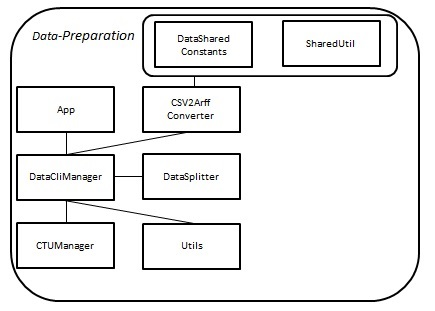
\includegraphics[width=0.65\textwidth]{images/Schema_Data_Preparation.jpg}
 \caption{Schema Data-Preparation}
 \label{fig:schema_data_preparation}
\end{figure}


\subsection{IDS Teil} \label{subsec:VorgehenIDS}

Im Intrusion Detection System kann der Nutzer zwischen mehreren Classifiern auswählen.
Hat der Nutzer einen Classifier ausgewählt und die Parameter gesetzt, trainiert das IDS auf dem in der Data-Preparation vorbereiteten Trainings-Datensatz und testet anschließend auf dem Test-Datensatz.
Es ist auch möglich nur ein Training oder nur einen Test durchzuführen.
Dies kann manchmal hilfreich sein, weil die einzelnen Rechnenschritte recht
zeitintensiv sein können.
Diese Option hat also nur praktische Zwecke.
Nachdem das IDS getestet hat, evaluiert es die Testergebnisse.
Die Resultate der Evaluierung, die Berechnung der Metriken True Positive, True
Negative, False Positive, False Negative, etc. werden sowohl in Text- als auch in
grafischer Form hinterlegt, um den Nutzer einen Überblick zu verschaffen.

Der Nutzer kann die Ausführung des IDS noch weiter einstellen.
Es gibt eine Option um einen Teil der Attribute, die in der ARFF Datei vom Typ
\textit{numeric} als \textit{nominal} zu interpretieren.
Wie im vorigen Abschnitt~\ref{subsec:VorgehenDatenaufbereitung} beschrieben,
wurden vorher einige der Attribute von \textit{nominal} zu \textit{numeric}
konvertiert, um Speicherplatz zu sparen.
Dies kann aber die Arbeit des IDS beeinflussen.
Es wäre möglich, dass sich dadurch die Berechnung des nächsten Nachbarn ändert.

Die nachfolgende Abbildung~\ref{fig:schema_ids} gibt einen detaillierten Überblick über den Aufbau des Intrusion Detection Systems. \\
Dabei sollte auffallen, dass wie schon einige Mal angedeutet auch die
Implementierung des IDS Systems die Trennung von Training(training) und
Test(evaluation) wiederspiegelt.

Der Training Teil besteht hauptsächlich aus Wrappern fuer die Weka Classifier,
um den Zugriff und die Speicherung von diesen zu erleichtern und Helfern, die
die Berechnung der Classifier anpassen auf unseren CTU Datensatz.
Eine dieser JAVA Klassen zur Anpassung ist die Klasse \textit{CTUIBk}.
Diese ist abgeleitet vom normalen \textit{nearest Neighbour WEKA classifier}.
Er passt die Prediction des normalen Classifiers an, indem er die ursprünglichen
drei Klassen, die der CTU-Datensatz hat, auf zwei Klassen runterrechnet, weil
wir fuer unsere Metriken, die in Abschnitt~\ref{subsubsec:WerteMetriken} näher
betrachtet werden, nur betrachten, ob eine Instanz normales oder Botnet
Verhalten darstellt.
Für die meisten Fälle rechnet dafür diese Klasse die Wahrscheinlichkeit heraus,
dass eine Instanz als Hintergrund klassifiziert wird, indem die
Wahrscheinlichkeit auf $0$ gesetzt wird.
Dafür werden die beiden anderen Wahrscheinlichkeiten entsprechnend vergrößert, wenn
sie nicht selbst $0$ sind.

\begin{figure}[ht]
 \centering
 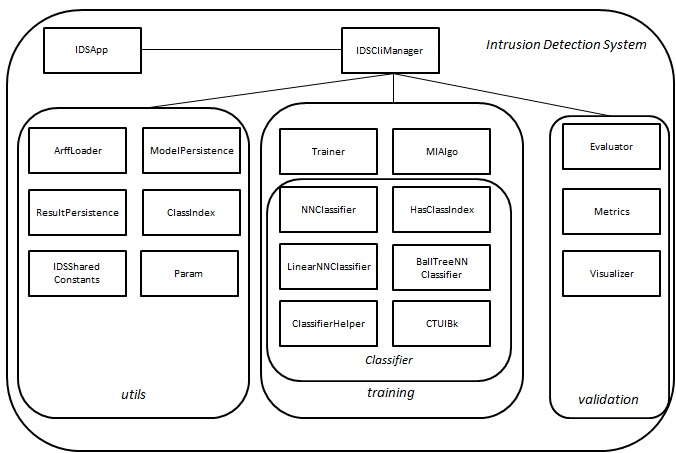
\includegraphics[width=1\textwidth]{images/Schema_IDS.jpg}
 \caption{Schema IDS}
 \label{fig:schema_ids}
\end{figure}

\section{Machine Learning}
\subsection{Classifier}
Für das IDS wurden die Classifier implementiert.


\end{document}

% Wie ist das IDS aufgebaut? (ggf. Schema einfügen)
% Was ist der NN-Algorithmus?
% Warum haben wir diesen Algorithmus gewählt?
% Wie wird dieser Algorithmus auf den Datensatz angewandt?
